\documentclass{report}

\usepackage[fleqn]{amsmath}
\usepackage{amssymb}
\usepackage{setspace}
\usepackage{enumitem}
\usepackage{fontspec}
\usepackage{titlesec}
\usepackage{nicematrix}
\usepackage{multicol}
\usepackage[total={6.6in,9.2in}]{geometry}

\usepackage{xparse}
\ExplSyntaxOn
%Thanks, Andrew! This looks way better than my previous example. :) 
\NewDocumentCommand\alotofdots{ D(){\ldotp} O{3}}
{\mathinner{\prg_replicate:nn{#2}{#1}}}
\ExplSyntaxOff

\setmainfont{Times New Roman}

\title{\Huge{\textbf{Coordinate Transformation}}}
\author{Melvin Chia}
\date{21 June 2023}

\setcounter{chapter}{3}

\titleformat{\chapter}[display]
{\normalfont\huge\bfseries}{\chaptertitlename\ \thechapter}{20pt}{\Huge}

% this alters "before" spacing (the second length argument) to 0
\titlespacing*{\chapter}{0pt}{0pt}{40pt}

\begin{document}
\maketitle

\onehalfspacing

\chapter{Coordinate Transformation}

\section{Translation of Axes}
The coordinates of points and the equation of curves are for certain axes. For
example, in the circle shown below, its center is at $(3, 2)$ in the coordinate
system $xOy$, and its equation is $(x - 3)^2 + (y - 2)^2 = 5$. If we were to
use the coordinate system $x'Oy' (O'x' // Ox, O'y' // Oy)$, they would become
$(3, 2)$ and $x'^2 + y'^2 = 5$ respectively.

\begin{multicols}{2}

    That is to say, for the same point or the same curve, the coordinates of the
    point and the equation of the curve would be different if different coordinate
    systems were chosen. As we can see in the example on the right, changing the
    coordinate system to a more suitable one can simplify the equation of the
    curve, hence making it easier to study the properties of the curve. \\
    \vspace{1em} Without changing the direction and the unit of length of the axes
    while changing only the position of the origin, this kind of transformation is
    called \textbf{translation of axes}. \columnbreak

    \begin{center}
        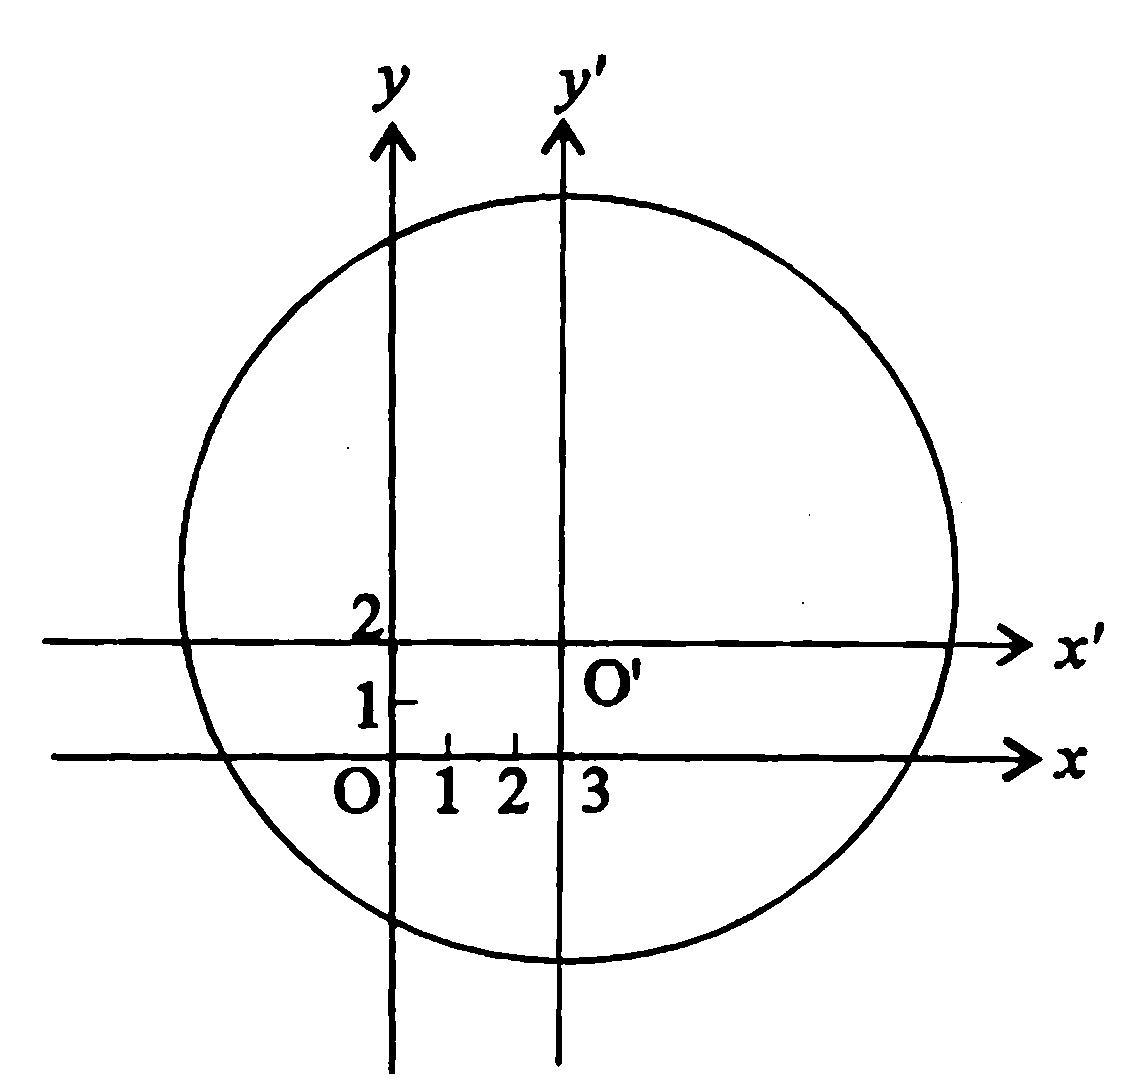
\includegraphics[scale=0.3]{./assets/fig1}
    \end{center}
\end{multicols}
\vspace{-1em}
Here we study the relationship between the coordinates of a point in two
different coordinate systems when performing a translation.

Let the coordinates of $O'$ at the original coordinate system $xOy$ be $(h,
    k)$, translate the axes with $O'$ as the origin, and create a new coordinate
system $x'O'y'$.
\begin{multicols}{2}
    As shown in the figure on the right, the coordinates of an arbitrary
    point $P$ in the original coordinate system are $(x, y)$, and its coordinates
    in the new coordinate system are $(x', y')$, the perpendicular foot from $P$ to
    the $x$-axis and the $x'$-axis are $M$ and $N$ respectively. We can see that,
    \begin{flalign*}
        x & = OH + HM \\
          & = h + x'  \\
        y & = OK + KN \\
          & = k + y'
    \end{flalign*}
    \begin{center}
        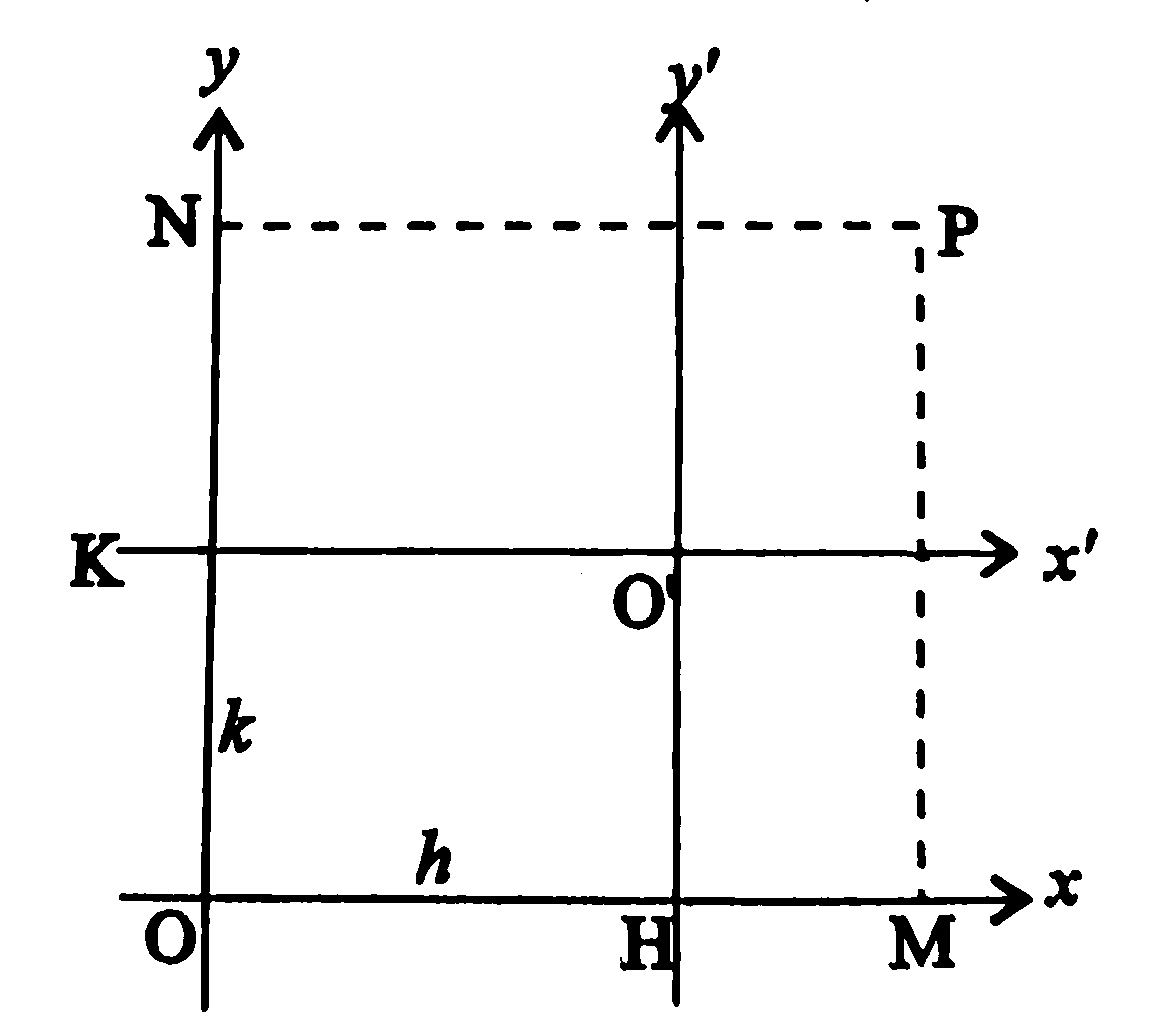
\includegraphics[scale=0.15]{./assets/fig2}
    \end{center}
\end{multicols}

\newpage
Hence the coordinates of $P$ in the original and the new coordinate systems has
the following relationship,

\begin{center}
    \fbox{\begin{minipage}{15em}
            \vspace{-1.2em}
            \begin{equation*}
                x = x' + h,\ y = y' + k
            \end{equation*}
            \vspace{-1.8em}
        \end{minipage}}
\end{center}
The formula above is called the \textbf{translation formula}.

\begin{enumerate}[label=\textbf{Example \arabic*}, leftmargin=*]
    \item Translate the axes, move the origin to $O'(3, -4)$ (as shown in the diagram
          below), find the new coordinates of the following points:

          $O(0, 0)$, $A(3, -4)$, $B(5, 2)$, $C(3, -2)$.
          \begin{enumerate}[label=\textbf{Sol.}, leftmargin=-0em, labelsep=1.2cm]
              \item Substituting the original coordinates of the given points into
                    \begin{flalign*}
                        x & = x' + 3 \\
                        y & = y' - 4
                    \end{flalign*}
                    We get the new coordinates of them:
                    \begin{flalign*}
                        O'(-3, 4),\ A'(0, 0),\ B'(2, 6),\ C'(0, 2)
                    \end{flalign*}
          \end{enumerate}
\end{enumerate}
\section{Simplifying Quadratic Equation of Two Variables by Translation of Axes}

Now, we study how choose the coordinate system to simplify the equation. First,
take a look at the following example.

\begin{enumerate}[label=\textbf{Example \arabic*}, leftmargin=*, start=2]
    \item Translate the axes and simplify the equation $x^2 - y^2 + 8x - 14y - 133 = 0$.
          \begin{enumerate}[label=\textbf{Sol. \arabic*}, leftmargin=-0em, labelsep=0.9cm]
              \item Substitute $x = x' + h$ and $y = y' + k$ into the equation, we get
                    \begin{flalign*}
                        {(x' + h)}^2 - {(y' + k)}^2 + 8(x' + h) - 14(y' + k) - 133 & = 0
                    \end{flalign*}
                    That is
                    \begin{flalign*}
                        x'^2 - y'^2 + (2h + 8)x' - (2k + 14)y' + h^2 - k^2 + 8h - 14k - 133 & = 0 \ \alotofdots(\cdotp)[6]\ (1) &
                    \end{flalign*}
                    Let $2h + 8 = 0$ and $2k + 14 = 0$, we get $h = -4$ and $k = -7$.
                    \begin{flalign*}
                         & \text{Substitute them into $(1)$, we get} & x'^2 - y'^2 = 100 &  &  &  &  &  &
                    \end{flalign*}
              \item Completing the square of the equation $x'^2 - y'^2 + 8x - 14y - 133 = 0$,
                    \begin{flalign*}
                        \text{We get} &  & x^2 + 8x - (y^2 + 14y)                                           & = 133 &  &  &  &  &  &              \\
                                      &  & (x + 4)^2 - 16 - (y + 7)^2 + 49                                  & = 133 &  &  &  &  &  &              \\
                        \text{Let}    &  & x' = x + 4,\ y' = y + 7,  \text{we get} \hspace{5em} x'^2 - y'^2 & = 100 &  &  &  &  &  & \hspace{5em}
                    \end{flalign*}
          \end{enumerate}
\end{enumerate}

\noindent Example 2 above shows that, for a quadratic equation of two variables that does not contain $xy$ term,
\begin{flalign*}
    ax^2 + by^2 + 2gx + 2fy + c = 0 \quad (\text{$a$ $b$ are not zero at the same time})
\end{flalign*}
We can translate the axes to simplify the equation.

\newpage
\subsection*{Exercise 4a}
\begin{enumerate}[leftmargin=*]
    \item Translate the axes, move the origin to $O'(4, 5)$. Find the new coordinates of
          the following points, and sketch the new coordinate system and each point:

          $A(3, -6)$, $B(7, 0)$, $C(-4, 5)$, $D(0, -8)$
    \item After the translation of the axes, the new coordinates of the point $(-1, 2)$
          is $(4, -3)$, find the original coordinates of the new point of origin.
    \item After the translation of the axes, the new coordinate of the points $(3, -3)$
          and $(-2, 2)$ are $(2, -1)$ and $(a, b)$ respectively. Find $a$ and $b$.
    \item After the translation of the axes, the new coordinates of the points $(-4, 2$
          and $(6, -2)$ are $(6, \alpha)$ and $(\beta, 4)$ respectively. Find $\alpha$
          and $\beta$.
    \item Translate the axes, move the origin to $O'(2, -3)$. Find the equation of $x^2 +
              y^2 - 4x + 6y - 3 = 0$ in the new coordinate system, and sketch the coordinates
          system and the graph.
    \item Using the translation of axes, simplify the following equations:
          \begin{enumerate}
              \item $x^2 + y^2 - 6x + 12y - 4 = 0$
              \item $8x^2 - 9y^2 - 16x + 36y - 77 = 0$
              \item $x^2 + y^2 - 2x + 6y - 6 = 0$
              \item $9x^2 + 4y^2 - 18x + 16y - 11 = 0$
          \end{enumerate}
    \item After the translation of the axes and moving the origin to $O'(1, -2)$, the new
          coordinates of the points $A$, $B$, $C$, and $D$ are $(-1, 1)$, $(0, -2)$, $(3,
              2)$, and $(2, 0)$ respectively, find their original coordinates, and sketch the
          original coordinate system and each point.
    \item After the transformation of the axes, the coordinates of the point $A$ changes
          from $(2, -1)$ to $(-2, 1)$. Find the coordinates the point of origin in the
          new coordinate system.
\end{enumerate}

\newpage
\section{Rotation of Axes}
Without changing the point of origin and the length unit of the coordinate
system, only rotate the coordinate system to the same direction by the same
degree around to the point of origin, we call this transformation
\textbf{rotation of axes}.

Let's derive the formula of the transformation of the coordinates under the
rotation of axes.

Let the angle of rotation of the axes be $\theta$, and pick an arbitrary point
$P$ on the plane, its coordinates in the coordinate system $xOy$ and $x'O'y'$
are $(x, y)$ and $(x', y')$ respectively, as shown in the figure on the right.

Draw $PS$, $PT$ perpendicular to the $x$-axis and the $x'$-axis respectively.
Connect $OP$, let $\angle POT = \alpha$, then
\begin{flalign*}
                  &  & x' & = \vert OP \vert \cos a                                        &   &  &  &  &  &  &  &  &  &  &  &  &  &  &  &  &  &  &  &  &  &  &  &  &  &  & \\
                  &  & y' & = \vert OP \vert \sin a                                        &                                                                                \\
    \text{Hence } &  & x  & = \vert OP \vert \cos (\alpha + \theta)                        &                                                                                \\
                  &  &    & = \vert OP \vert (\cos\theta\sin\alpha - \sin\theta\cos\alpha) &                                                                                \\
                  &  &    & = x'\cos\theta - y'\sin\theta                                  &                                                                                \\
                  &  & y  & = \vert OP \vert \sin (\alpha + \theta)                        &                                                                                \\
                  &  &    & = \vert OP \vert (\sin\theta\sin\alpha + \cos\theta\cos\alpha) &                                                                                \\
                  &  &    & = x'\sin\theta + y'\cos\theta
\end{flalign*}
That is,
\begin{center}
    \fbox{\begin{minipage}{15em}
            \vspace{-1.2em}
            \begin{flalign*}
                \ \ x = x'\cos\theta - y'\sin\theta \\
                y = x'\sin\theta + y'\cos\theta
            \end{flalign*}
            \vspace{-1.8em}
        \end{minipage}}
\end{center}

The formula above is called the \textbf{rotation formula}.

\begin{enumerate}[label=\textbf{Example \arabic*}, start=3, leftmargin=*]
    \item Rotating the axes by $\dfrac{\pi}{6}$, find the coordinate of the point
          $P\left(-1, \sqrt{3}\right)$ in the new coordinate system.
          \begin{enumerate}[label=\textbf{Sol.}, leftmargin=-0em, labelsep=1.2cm]
              \item Substitute $\theta = \dfrac{\pi}{6}$, $x = -1$, $y = \sqrt{3}$ into the
                    rotation formula, we get
                    \begin{flalign*}
                                                           &  & -1         & = x'\cos\dfrac{\pi}{6} - y'\sin\dfrac{\pi}{6}              &  &  &  &  &  & \\
                                                           &  & -2         & = \sqrt{3}x' - y' \ \alotofdots(\cdots)[6]\ (1)                             \\
                        \text{And }                        &  & \sqrt{3}   & = x'\sin\dfrac{\pi}{6} + y'\cos\dfrac{\pi}{6}                               \\
                                                           &  & 2\sqrt{3}  & = x' + \sqrt{3}y' \ \alotofdots(\cdots)[6]\ (2)                             \\
                        (1) \times \sqrt{3}\text{, we get} &  & -2\sqrt{3} & = 3x' - \sqrt{3}y' \ \alotofdots(\cdots)[5]\cdot\cdot\ (3)                  \\
                        (2) + (3), \text{we get}           &  & x'         & = 0                                                                         \\
                                                           &  & y'         & = 2
                    \end{flalign*}
                    $\therefore$ The coordinate of the point $P$ in the new coordinate system is $(0, 2)$.
          \end{enumerate}
\end{enumerate}

\newpage
\begin{enumerate}[label=\textbf{Example \arabic*}, start=4, leftmargin=*]
    \item Rotate the axes by $\dfrac{\pi}{3}$, find the equation of the curve $2x^2 -
              \sqrt{3}xy + y^2 = 10$ in the new coordinate system.
          \begin{enumerate}[label=\textbf{Sol.}, leftmargin=-0em, labelsep=1.2cm]
              \item Substitute $\theta = \dfrac{\pi}{3}$ into the rotation formula, we get
                    \begin{flalign*}
                        x & = x'\cos\dfrac{\pi}{3} - y'\sin\dfrac{\pi}{3} \\
                          & = \dfrac{1}{2}x' - \dfrac{\sqrt{3}}{2}y'      \\
                        y & = x'\sin\dfrac{\pi}{3} + y'\cos\dfrac{\pi}{3} \\
                          & = \dfrac{\sqrt{3}}{2}x' + \dfrac{1}{2}y'
                    \end{flalign*}
                    Substitute into the original equation, we get the equation of the curve in the new coordinate system
                    \begin{flalign*}
                        2\left(\dfrac{1}{2}x' - \dfrac{\sqrt{3}}{2}y'\right)^2 - \sqrt{3}\left(\dfrac{1}{2}x' - \dfrac{\sqrt{3}}{2}y'\right)\left(\dfrac{\sqrt{3}}{2}x' + \dfrac{1}{2}y'\right) + \left(\dfrac{\sqrt{3}}{2}x' + \dfrac{1}{2}y'\right)^2 & = 10
                    \end{flalign*}
                    Simplifying the equation above, we get \qquad $\dfrac{x'^2}{20} + \dfrac{y'^2}{4} = 1$.
          \end{enumerate}
\end{enumerate}

\subsection*{Exercise 4b}
\begin{enumerate}[leftmargin=*]
    \item Let the angle of rotation $\theta = -\dfrac{\pi}{4}$, find the original
          coordinates of two points $A(-3, 2)$ and $B(1, 0)$ in the new coordinate
          system.
    \item Let the angle of rotation $\theta = \dfrac{\pi}{6}$, find the new coordinates
          of two points $C(2, -1)$ and $D(0, 1)$ in the original coordinate system.
    \item Transform the following equations by rotating the axes by the given angle:
          \begin{enumerate}
              \item $x + y = 0$, \qquad\qquad\qquad\hspace{1.4em} $\theta = \dfrac{\pi}{4}$
              \item $x - y = 0$, \qquad\qquad\qquad\hspace{1.4em} $\theta = \dfrac{\pi}{2}$
              \item $x^2 + y^2 = 9$, \qquad\qquad\qquad\hspace{0.7em}$\theta = -\dfrac{\pi}{3}$
              \item $x^2 - 2\sqrt{3}xy + 3y^2 = 8$, \qquad $\theta = -\dfrac{\pi}{3}$
          \end{enumerate}
    \item If the origin of the coordinate system does not change,
\end{enumerate}

\end{document}